\section{Speculation}
\label{sec:speculation}
Whenever we move an instruction above a branch it is control-flow dependent on, we consider this instruction to be \textit{speculatively} executed~\cite{chang95}. When speculating during compilation, we typically try to tailor the control flow of the program toward the actual behavior we expect during runtime. The most common types of speculations include loads, computations, and stores. While these may increase performance in certain cases, they each come with considerations and hazards one has to be aware of. In this section, we will study the concepts and heuristics behind speculative execution. 

\subsection{Superblock Structure}
\label{sec:superblock_struct}
If we consider the control flow of a program, a superblock~\cite{10.1145/161541.159765} is a consecutive sequence of instructions that is always entered at the top-most basic block but may be left at arbitrary and multiple points. When forming a superblock, we try to anticipate the future control flow of the program during run time by either profiling it with synthetic data or other means~\cite{639244}. An example of how the profile of the program seen in listing \ref{ls:ls_c_chang_full_default} may look can be seen in the weighted control flow graph in figure~\ref{fig:controlflow_full}~\cite{chang95}. The numbers on the edges correspond to the frequency at which the respective control flow path was taken during execution. 

\begin{center}
    \begin{minipage}{.45\textwidth}
            \begin{lstlisting}[style=CStyle]
avg = 0;
weight = 0;
count = 0;

while (ptr != NULL) {
	count++;
	if(ptr->wt < 0) {
		weight -= ptr->wt;
	} else {
		weight += ptr->wt;
	}
	ptr = ptr->next;
}

if(count !=0) {
	avg = weight / count;
}
\end{lstlisting}
        \captionsetup{type=listing}
        \captionof{lstlisting}[C Code for Example CFG]{C Code for Example CFG.}
        \label{ls:ls_c_chang_full_default}
    \end{minipage}
\end{center}

\clearpage
\begin{center}
    \begin{minipage}{.69\textwidth}
        \begin{figure}[H]
            \centering
            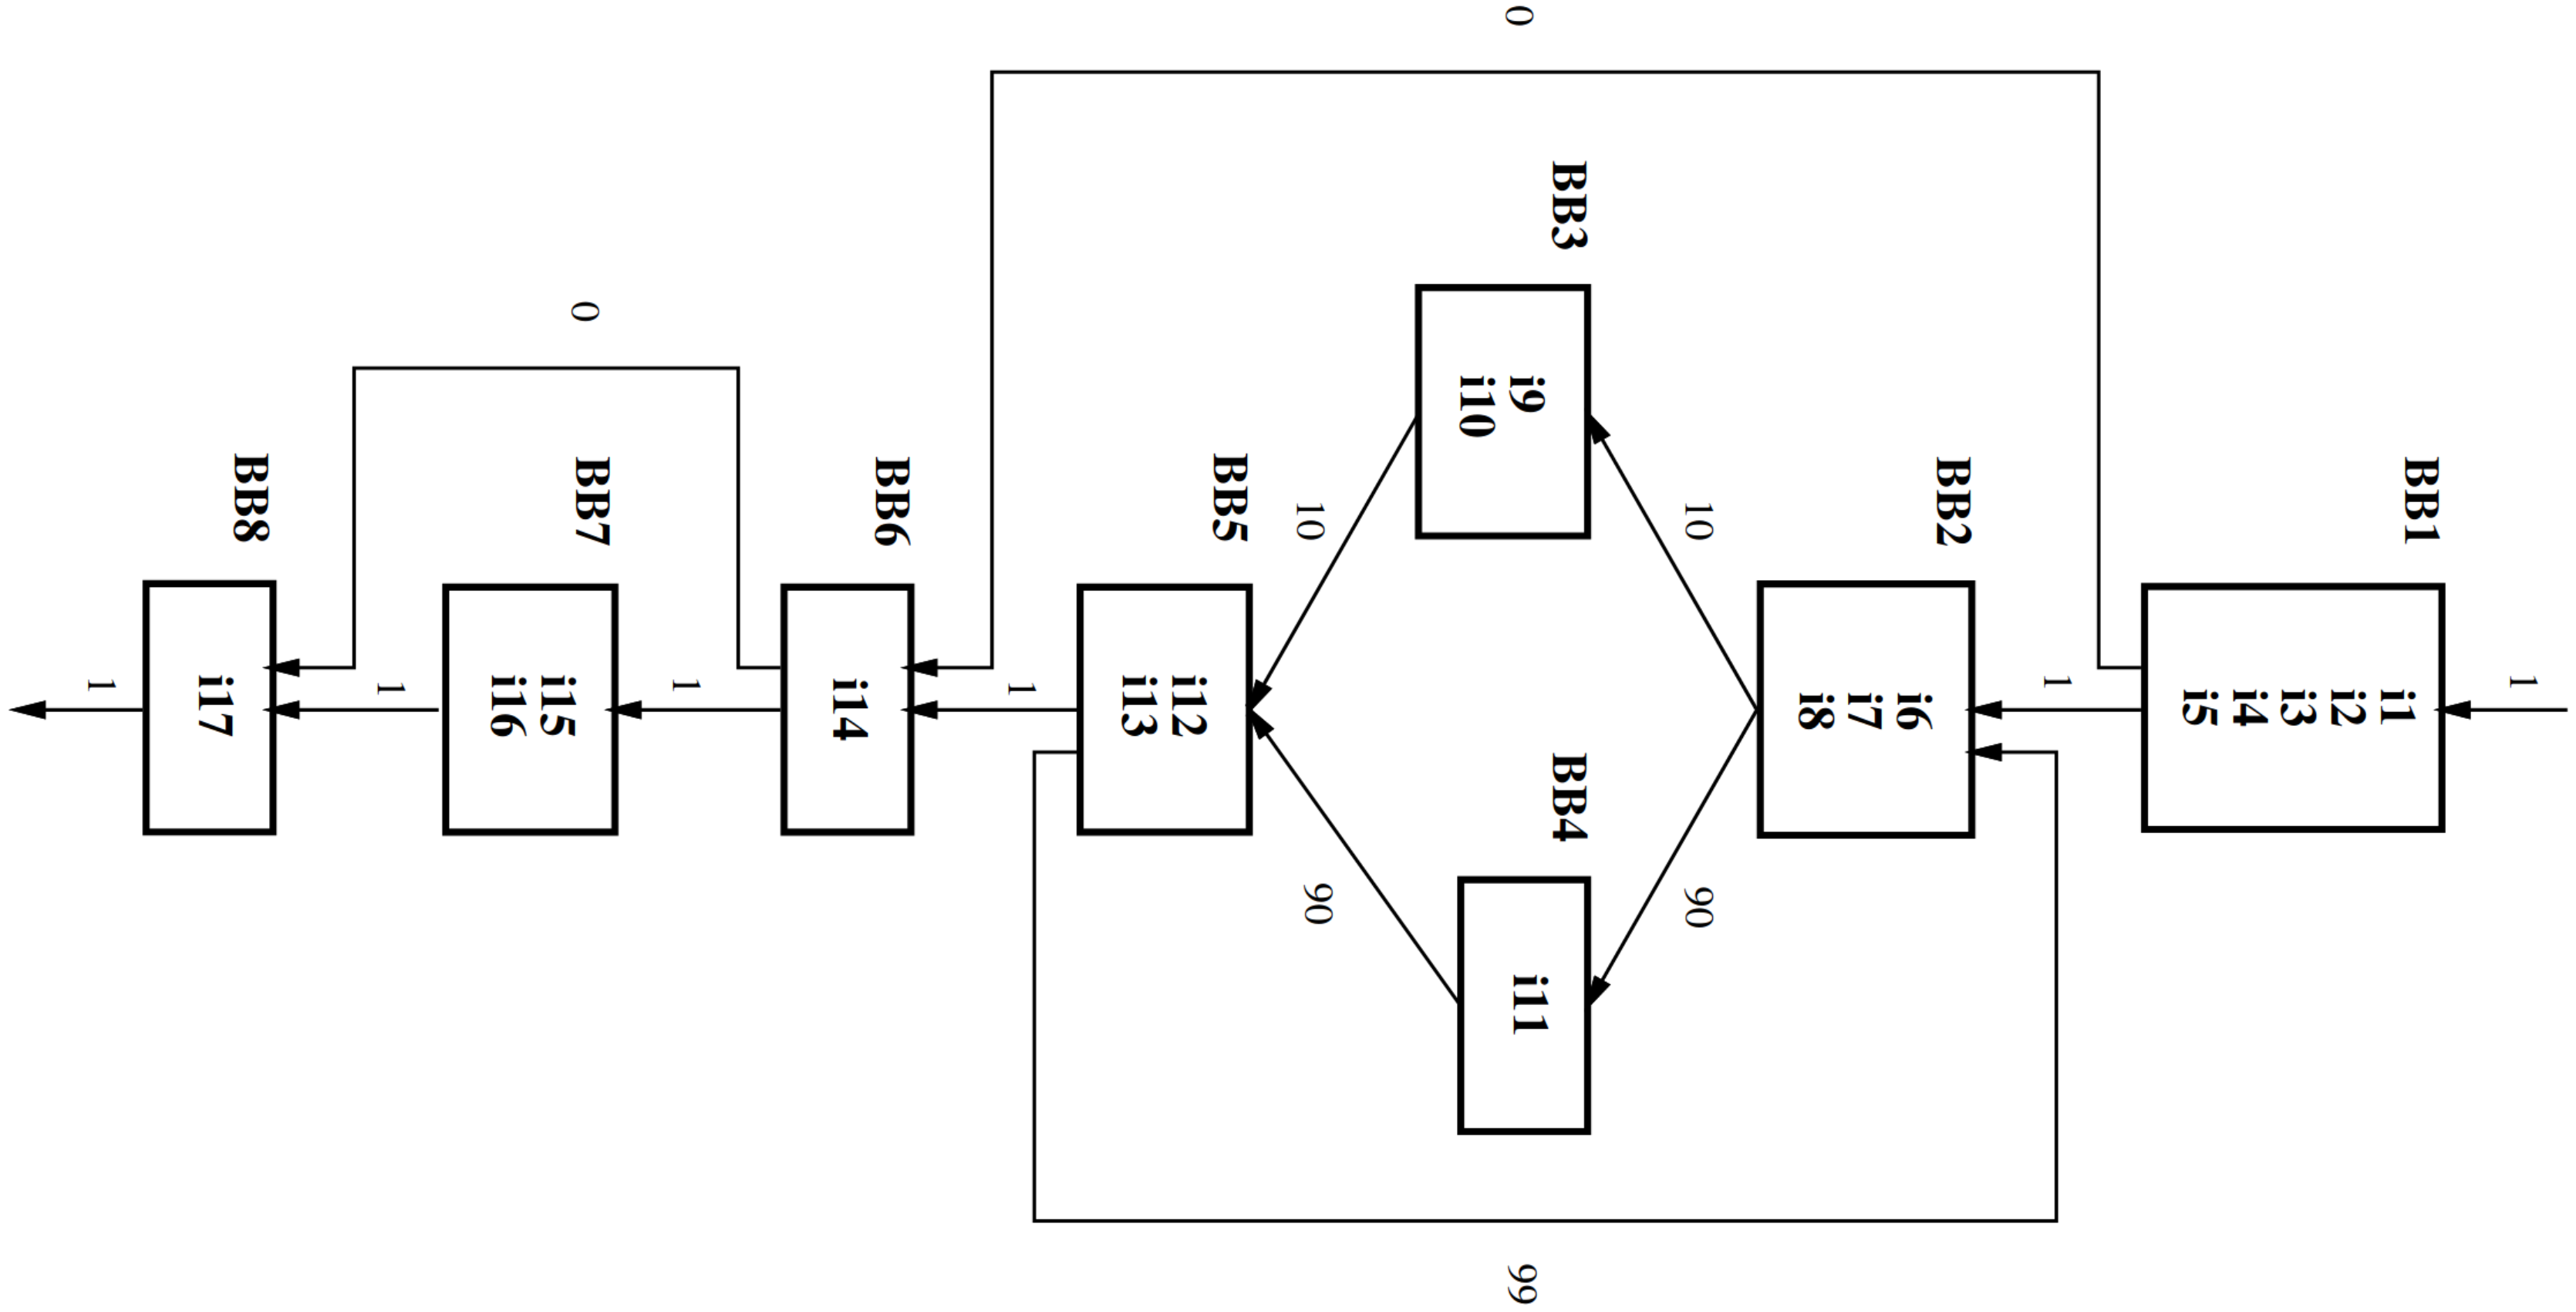
\includegraphics[width=1\linewidth, angle=90]{src//figure//image/image_chang_default_cfg.png}
            \caption[Example Control Flow Graph with Profiling Data]{An example control flow graph with profiling data. Courtesy of Chang et al.~\cite{chang95}.}
            \label{fig:controlflow_full}
\end{figure}
    \end{minipage}\hfill
    \begin{minipage}{.31\textwidth}
    \begin{lstlisting}[style=AsmStyle]
    ldr r1, _ptr   ; I1
    mov r7, 0      ; I2
    mov r2, 0      ; I3
    mov r3, 0      ; I4
    beq L3, r1, 0  ; I5
L0:
    add r2, r2, 1  ; I6
    ldr r4, 0[r1]  ; I7
    bge L1, r4, 0  ; I8
    sub r3, r3, r4 ; I9
    br L2          ; I10
L1:
   add r3, r3, r4  ; I11
L2:
   ldr r1, 4[r1]   ; I12
   bne L0, r1, 0   ; I13
L3:
    beq L4, r2, 0  ; I14
    div r7, r3, r2 ; I15
    str _avg r7    ; I16
L4: 
\end{lstlisting}

%     ldr     r1, =_ptr            ; 2. Load address of _ptr
%     ldr     r1, [r1]             ; 3. Load value of _ptr into r1
%     str     r1, [sp, #12]        ; 4. Store ptr on stack
%     mov     r7, #0               ; 5. avg = 0
%     mov     r2, #0               ; 6. count = 0
%     mov     r3, #0               ; 7. weight = 0
%     ldr     r0, [sp, #12]        ; 8. Load ptr from stack
%     cmp     r0, #0               ; 9. Compare ptr to 0
%     beq     L3                   ; 10. If ptr == 0, branch to L3
% L0:
%     add     r2, r2, #1           ; 11. count = count + 1
%     ldr     r4, [r0]             ; 12. Load ptr->wt into r4
%     cmp     r4, #0               ; 13. Compare ptr->wt with 0
%     blt     L1                   ; 14. If ptr->wt < 0, branch to L1
%     add     r3, r3, r4           ; 15. weight = weight + ptr->wt
%     b       L2                   ; 16. Branch to L2
% L1:
%     sub     r3, r3, r4           ; 17. weight = weight - ptr->wt
% L2:
%     ldr     r0, [r0, #4]         ; 18. ptr = ptr->next
%     cmp     r0, #0               ; 19. Compare ptr to 0
%     bne     L0                   ; 20. If ptr != 0, loop back to L0
% L3:
%     cmp     r2, #0               ; 21. Compare count to 0
%     beq     L4                   ; 22. If count == 0, skip division
%     div     r7, r3, r2           ; 23. avg = weight / count
%     ldr     r0, =_avg            ; 24. Load address of _avg
%     str     r7, [r0]             ; 25. Store avg into _avg
% L4:
%     add     sp, sp, #20          ; 26. Deallocate stack space

        \captionsetup{type=listing}
        \captionof{lstlisting}[\texttt{ARM} Assembly Code of Example CFG]{\texttt{ARM} Assembly Code of Example CFG.}
        \label{ls:ls_asmm_chang_full_default}
    \end{minipage}
\end{center} 


Figure \ref{fig:controlflow_side_enterance} shows the loop part of the program which consists of BB2, BB3, BB4, and BB5. In 90\% of the cases, we jump from BB2 to BB4 and BB5. Groups of blocks like this which frequently execute together are also called \textit{trace}. Our goal is to create a superblock from this trace to reduce bookkeeping complexity which typically arises during trace scheduling when we move instructions across side entrances. However, the edge from BB3 to BB5 is a side entrance into the trace. To remove it, we essentially tail duplicate BB5 by copying \texttt{I12} and \texttt{I13} seen in listing~\ref{ls:ls_asmm_chang_full_default}  to BB3' which now also forms a superblock by itself. We can omit \texttt{I10} since it was the branch instruction into BB5. Superblocks are not exclusively tools of speculation, rather they are also important for enabling other optimizations in compilers. 

\begin{center}
    \begin{minipage}{.38\textwidth}
        \begin{figure}[H]
            \centering
            \resizebox{1\textwidth}{!}{
            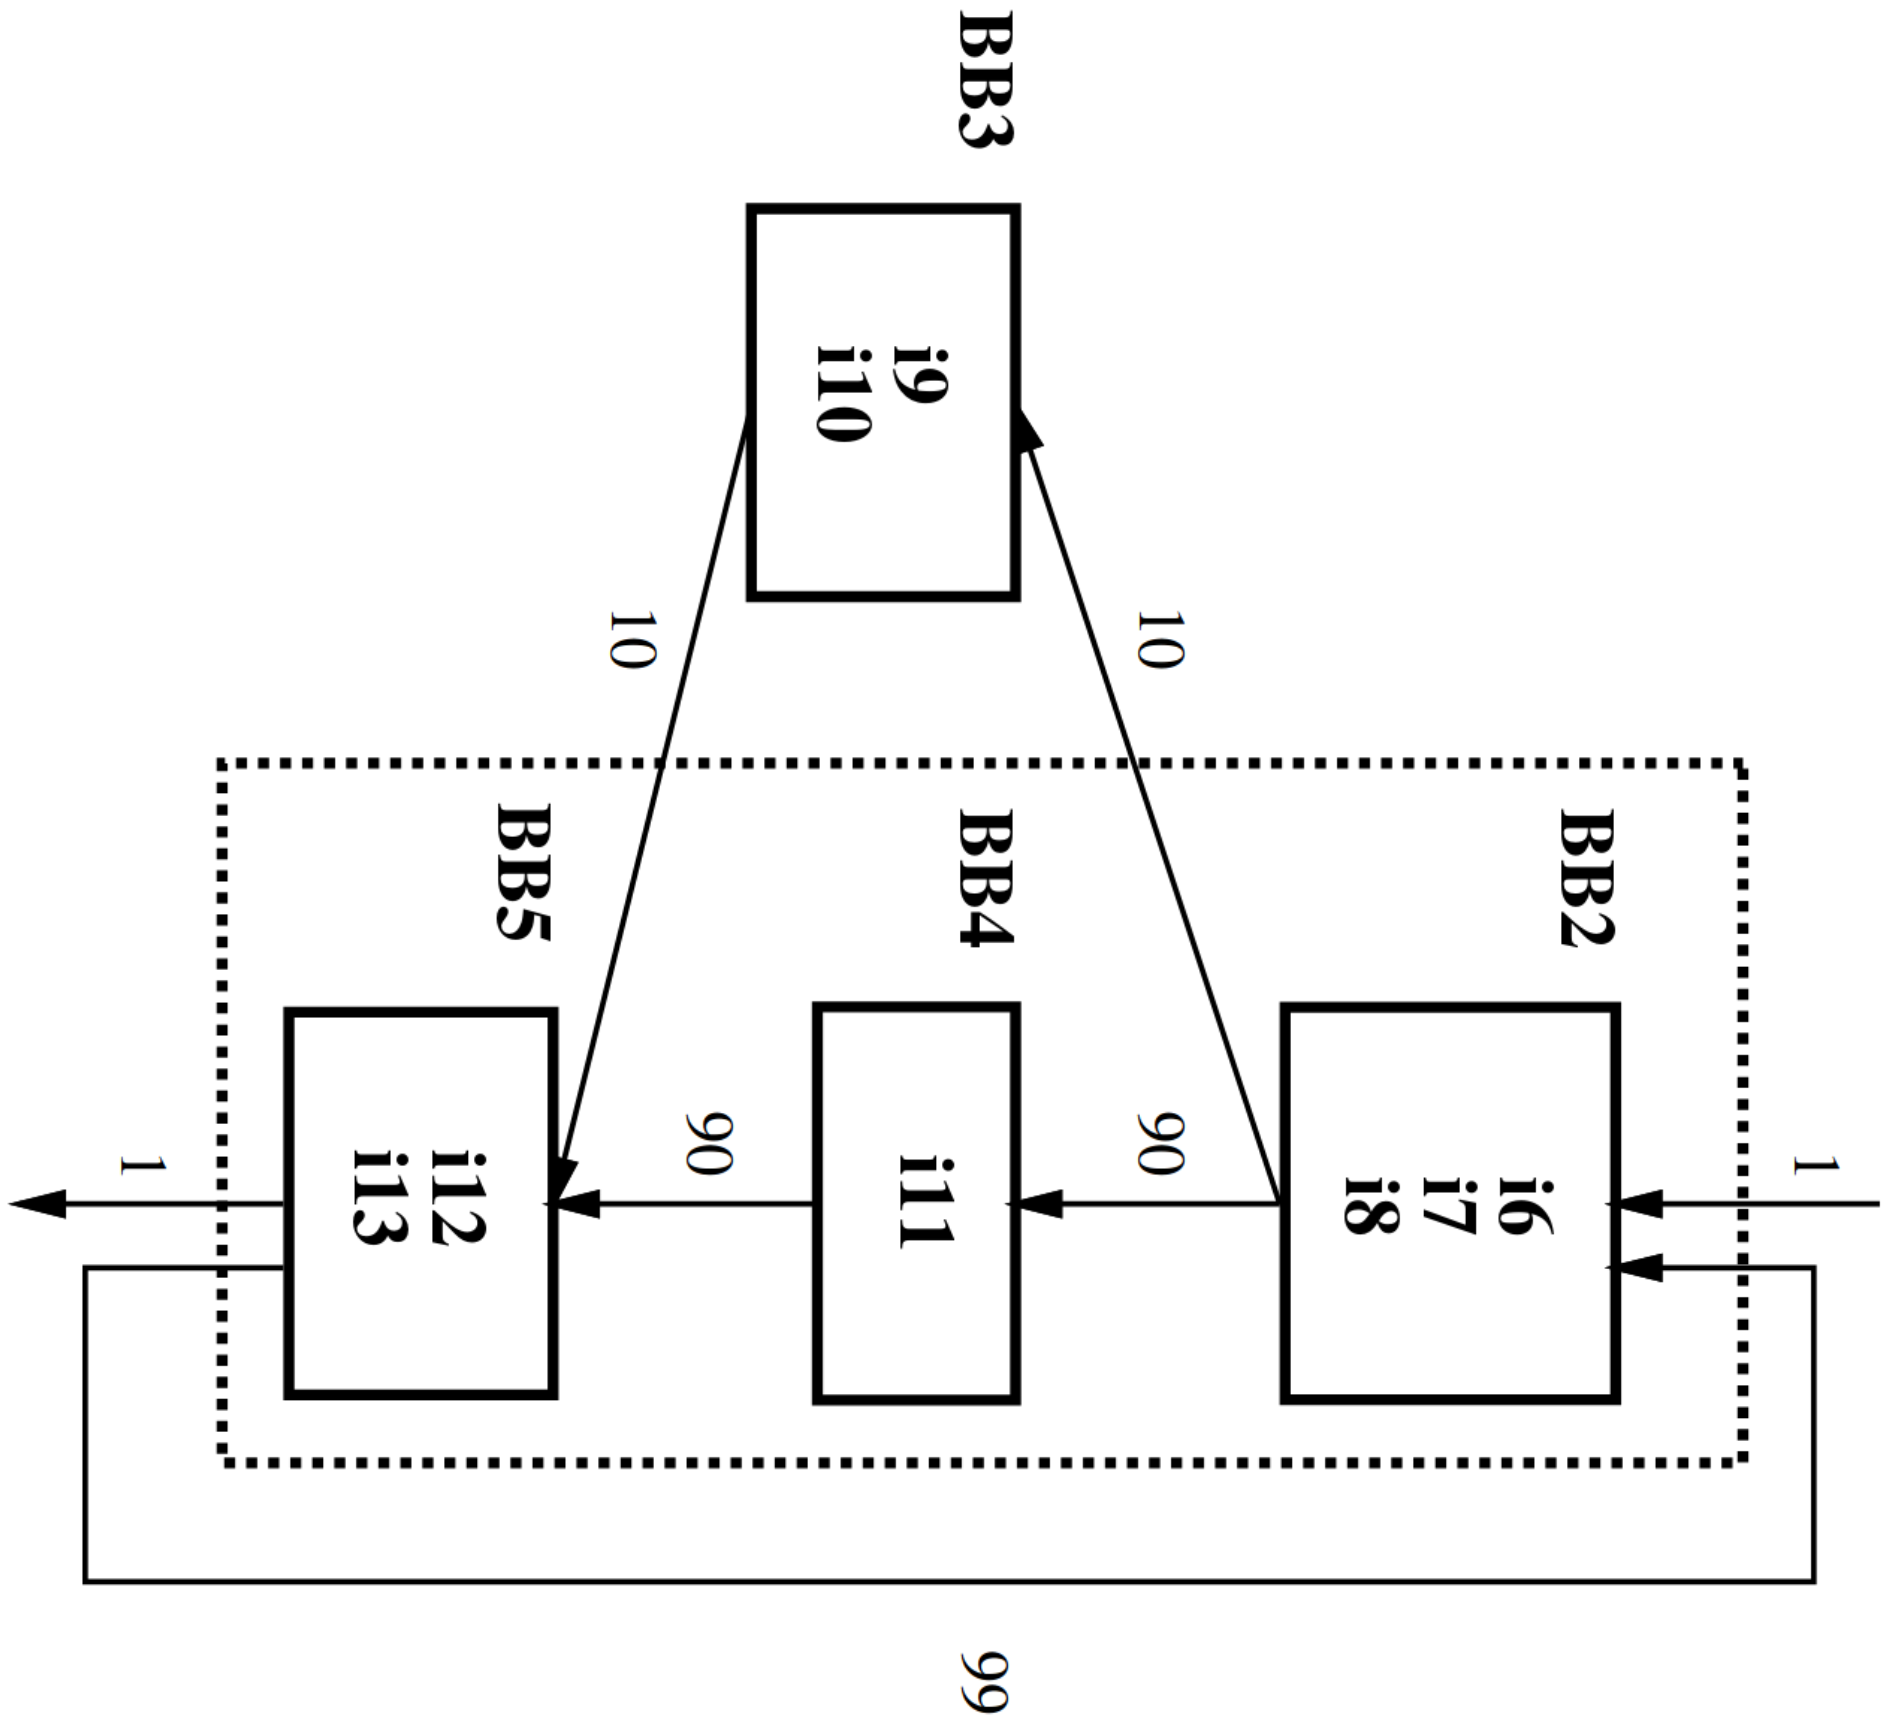
\includegraphics[width=\linewidth, angle=90]{src//figure//image/image_chang_loop_cfg.png}

        }
        \caption[Loop Part with Side Entrance]{Loop Part with Side Entrance. Courtesy of Chang et al.~\cite{chang95}.}
        \label{fig:controlflow_side_enterance}
\end{figure}
    \end{minipage}\hfill
    \begin{minipage}{.58\textwidth}
    \begin{figure}[H]
        \centering
        \resizebox{1\textwidth}{!}{
            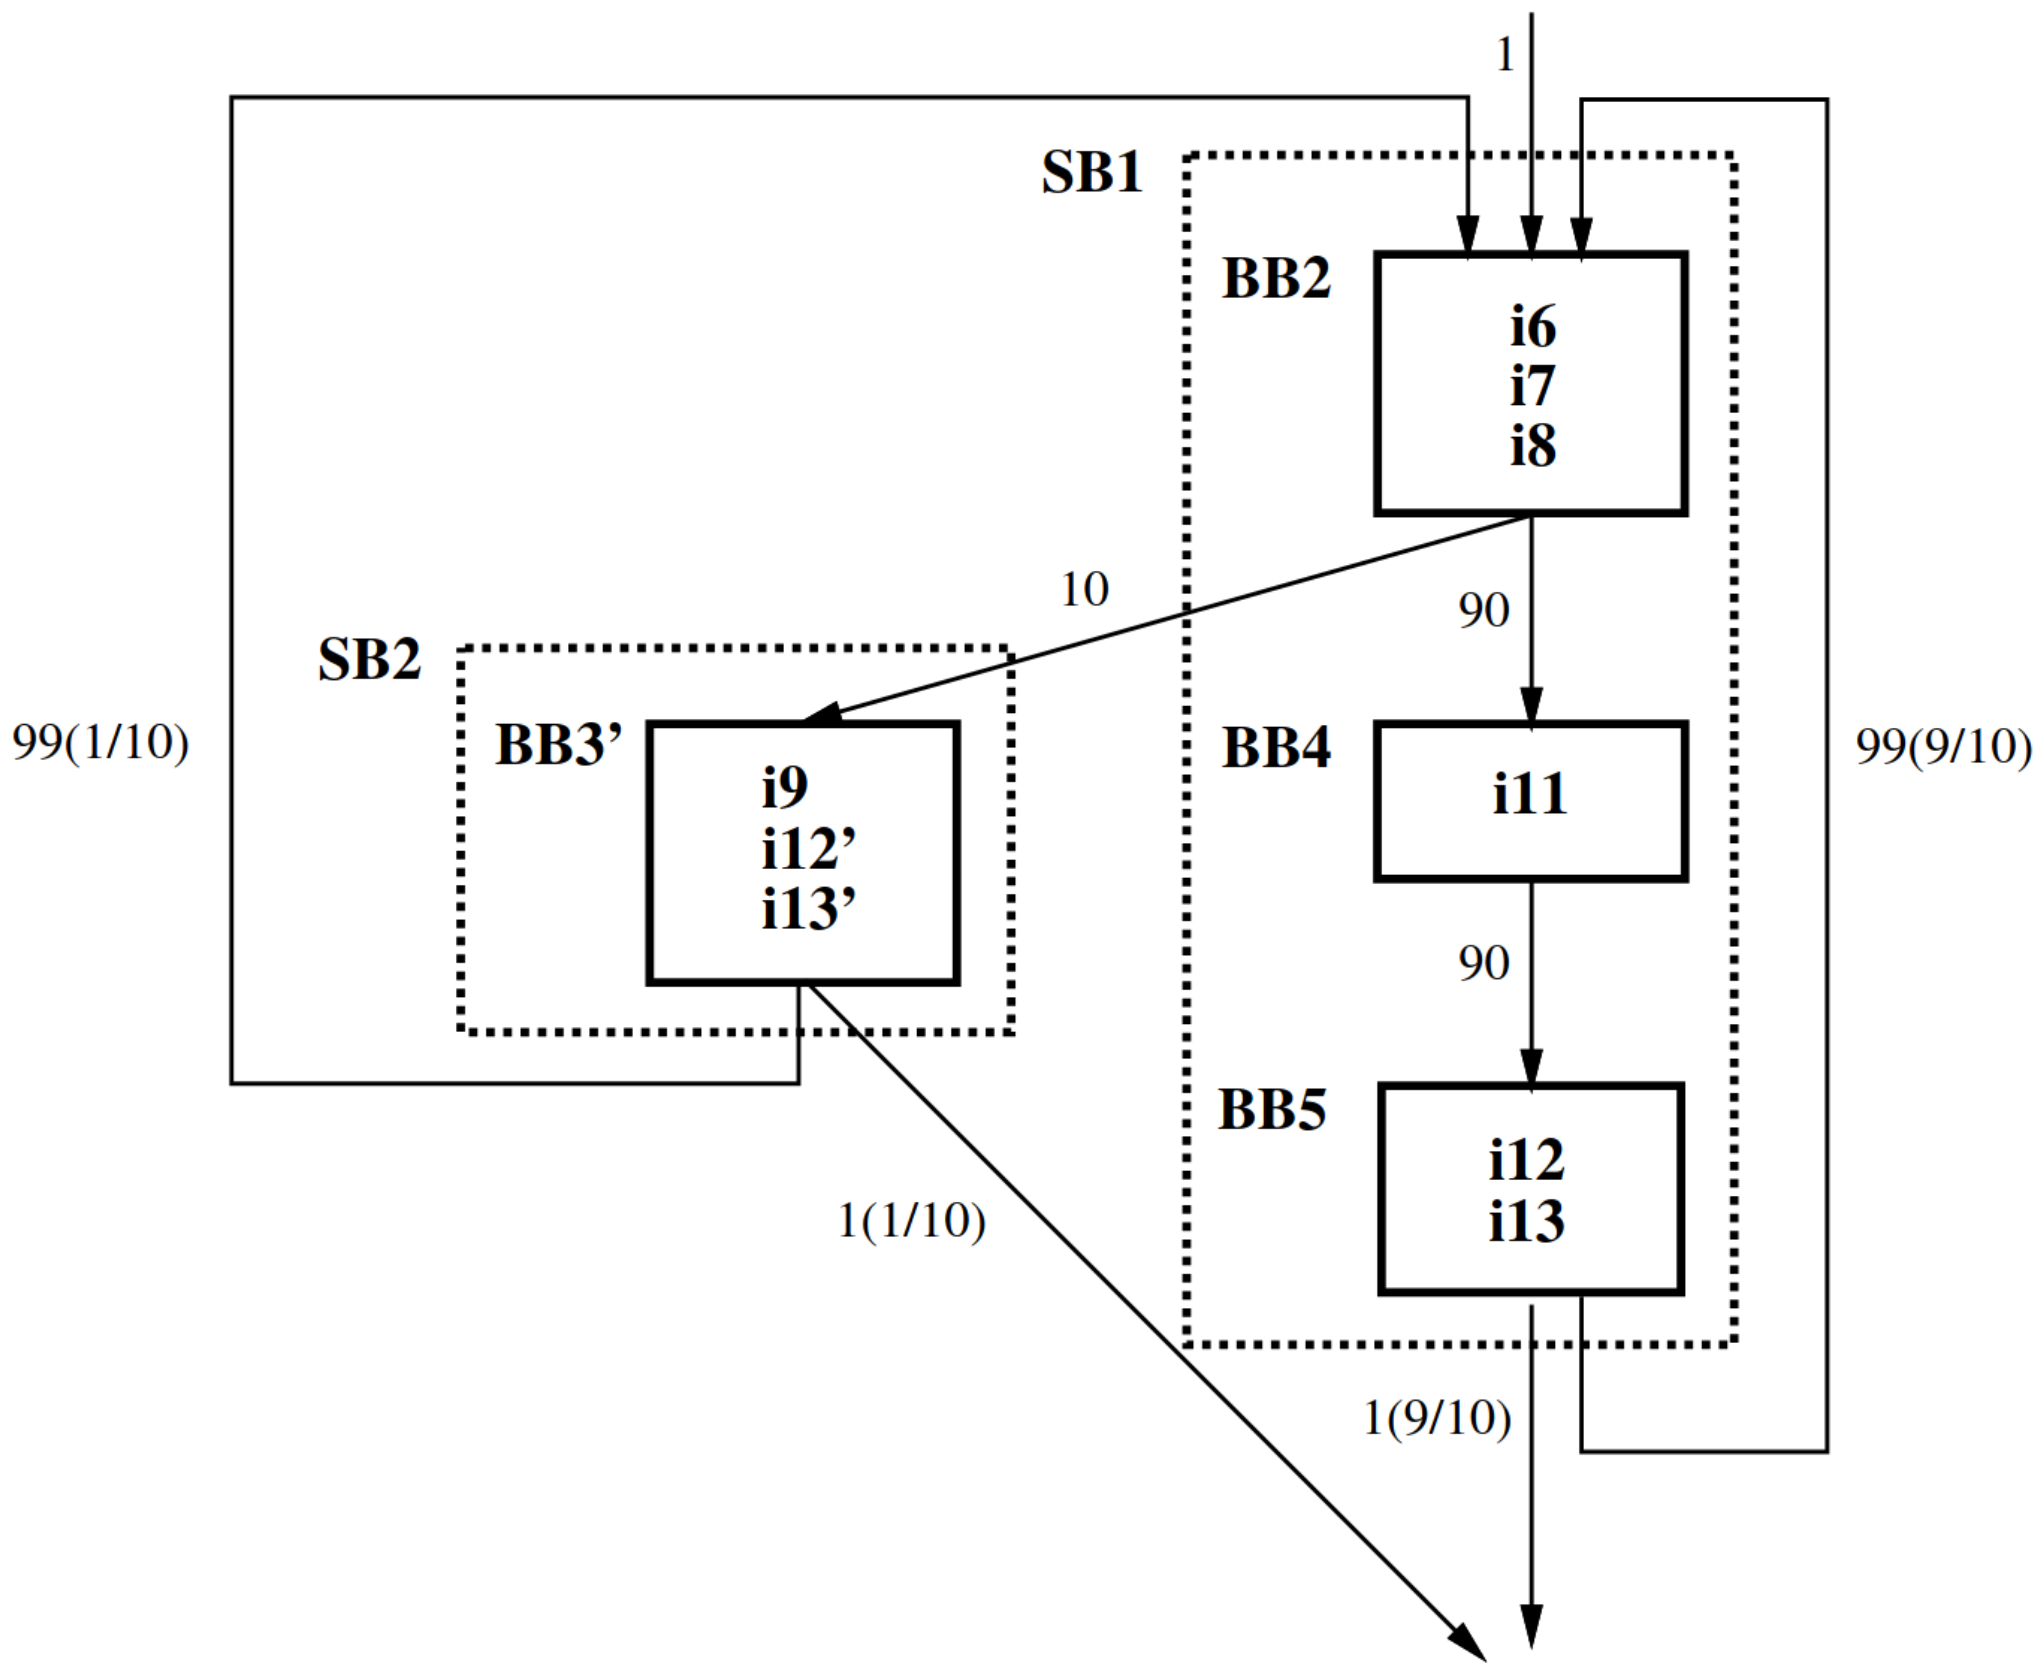
\includegraphics[width=0.5\linewidth]{src//figure//image/image_chang_sb_loop_cfg.png}

        }
        \caption[Loop Part Superblock Example]{The loop part of the program after Superblock creation. Courtesy of Chang et al.~\cite{chang95}.}
        \label{fig:controlflow_superblock}
\end{figure}
    \end{minipage}
\end{center} 


\subsection{Superblock Scheduling}
After the trace selection and the formation of superblocks, the compiler has to schedule the instructions to enable as much ILP as possible and the constraint of producing a save and correct program. This is done by building a graph that represents the dependencies among the instructions. The dependency graph is used during and subsequent list scheduling. The compiler may use heuristics and given instruction latencies to assign priorities to instructions which are \textit{ready} to produce a schedule that will use the available resources as efficiently as possible~\cite{chang95}. To enhance this further, the compiler needs to be able to move instructions above previous branches which is considered a speculation and will be discussed in section \ref{sec:spec_motion}. 

\subsection{Speculative Code Motion during Superblock Scheduling}
\label{sec:spec_motion}
In many cases, higher performance can be achieved by moving certain instructions either down or upward. However, in both cases, we have to retain the correctness of the original program. A variable or register is called \textit{live} if it holds a value that will be needed by other instructions.  For branch instructions, we can define \texttt{live-out(Br)} as the set of variables that may be used before being defined in case \texttt{Br} will be taken.

\subsubsection{Downward Motion}
Downward code motion, meaning moving an instruction \texttt{I} beneath a later instruction \texttt{Br} can always be applied if \texttt{Br} is not dependent on the result of \texttt{I}. In case the destination register of \texttt{I} is in \texttt{live-out(Br)}, we have to insert a copy of \texttt{I} between \texttt{Br} and its target to ensure correctness, as can be seen in listing~\ref{ls:ls_downward_default}

\begin{center}
    \begin{minipage}{.45\textwidth}
        \centering
        \begin{lstlisting}[style=AsmStyle]
    LDR     r1, [R2]
    CMP     r3, #0
    BEQ     Target
    ADD     r4, r1, r5
    ; ...
Target:
    SUB     r6, r1, r7
\end{lstlisting}
        \captionsetup{type=listing}
        \captionof{lstlisting}[Default Example Downward Motion]{Since \texttt{r1} is needed in the branch target of the \texttt{BEQ} instruction, \texttt{live-out(BEQ)} contains \texttt{r1}.}
        \label{ls:ls_downward_default}
    \end{minipage}\hfill
    \begin{minipage}{.45\textwidth}
        \centering
        \begin{lstlisting}[style=AsmStyle]    
    CMP     r3, #0
    BEQ     Target
    LDR     r1, [r2]
    ADD     r4, r1, r5
    ; ...
Target:
    @LDR     r1, [r2]@
    SUB     r6, r1, r7
\end{lstlisting}
        \captionsetup{type=listing}
        \captionof{lstlisting}[Downward Motion with Copy]{We can delay the \texttt{LDR} instruction by moving it downward. However, in case the \texttt{BEQ}-branch is taken, we need to load the correct value using a copy of the \texttt{LDR} instruction.}
    \end{minipage}
\end{center}

Although downward motion can be easily done, the cases where we will gain performance are limited.

\subsubsection{Restrictions for Upward Motion}
Moving an instruction from a point after a branch to a point before the branch is referred to as upward motion. Typically, one may try to schedule long-latency instructions early to reduce the critical path, for example in a superblock. Similar to other architectures, the division instruction \texttt{SDIV} is an example of such a long-latency instruction. As can be seen in listing ~\ref{ls:ls_upward_default}, depending on the input data, we may have to execute \texttt{SDIV}. Therefore it would be preferable to speculatively execute the division as can be seen in listing~\ref{ls:ls_upward_faulty}. However, the destination of \texttt{SDIV} (\texttt{r1}) is in \texttt{live-out(BEQ)} if it is taken, hence the speculation would alter the result if the compiler does not introduce compensation code, e.g. a copy of \texttt{r1} for the \texttt{taken} case. Additionally, \texttt{SDIV} may cause an exception since it was moved above the branch which checks the loaded value in \texttt{r1} to be zero. 

\begin{center}
    \begin{minipage}{.45\textwidth}
        \centering
        \begin{lstlisting}[style=AsmStyle]    
    LDR r1, [address]
    CMP r1, #0
    BEQ taken
    SDIV r1, #5, r1
    B end
taken:
    ADD r1, r1, #2
end:
\end{lstlisting}
        \captionsetup{type=listing}
        \captionof{lstlisting}[Default Example Upward Motion]{Depending on the input data, we may have to execute a division which typically takes many cycles in most architectures.}
        \label{ls:ls_upward_default}
    \end{minipage}\hfill
    \begin{minipage}{.45\textwidth}
        \centering
        \begin{lstlisting}[style=AsmStyle]
    ldr r1, [address]
    ldr r2, [address2]
    @sdiv r2, #5, r1@
    beq taken, r1, #0
    b end
taken:
    add r1, r2, #2
end:
\end{lstlisting}
        \captionsetup{type=listing}
        \captionof{lstlisting}[Faulty Upward Motion ]{The long-latency division was naively moved upwards. Depending on the input data, the program will now compute wrong results, because the destination register of the speculatively executed division \texttt{r1} is in \texttt{live-out(BEQ)}. In addition, \texttt{SDIV} may cause an unnecessary a divide-by-zero exception.}
        \label{ls:ls_upward_faulty}
    \end{minipage}
\end{center}

In general, we can formulate two restrictions one has to consider when applying speculation: 
\paragraph{Restriction 1:} The destination register of \texttt{I} is not in \texttt{live-out(Br)}. Hence, the result of \texttt{I} is not used before it is redefined when the branch was taken.
\paragraph{Restriction 2:} Instruction \texttt{I} will not cause an exception which will alter the program execution if \texttt{Br} is taken. 
\\ \\ 

 In combination with hardware support of the target, different speculation models typically result in dependence graphs which may allow the compiler to perform certain speculations during superblock scheduling. The code in listing~\ref{ls:ls_superblock_assembly} which corresponds to the program in listing~\ref{ls:ls_c_chang_full_default} which is courtesy of Chang et al. will serve as an example in the following sections to showcase increasingly aggressive speculation models. We assume a processing unit with universal functional units with a one-cycle latency for ALU instructions and a two-cycle load delay. The instruction labeled \texttt{I1} to \texttt{I12} belong to the superblock previously discussed in section~\ref{sec:superblock_struct}.
\begin{center}
        % \begin{lstlisting}[style=AsmStyle]
% 	ldr r1, _ptr
% 	mov r7, 0
% 	mov r2, 0
% 	mov r3, 0
% 	beq L3, r1, 0
% L0:
% 	add r2, r2, 1  ; I1
% 	ldr r4, 0[r1]  ; I2
% 	btl L1, r4, 0  ; I3
% 	add r3, r3, r4 ; I4
% 	ldr r5, 4[r1]  ; I5
% 	beq L3, r5, 0  ; I6
% 	add r2, r2, 1  ; I7
% 	ldr r6, 0[r5]  ; I8
% 	btl L1X, r6, 0 ; I9
% 	add r3, r3, r6 ; I10
% 	ldr r1, 4[r5]  ; I11
% 	bne L0, r1, 0  ; I12
% L3:
% 	beq L4, r2, 0
% 	div r7, r3, r2
% 	str _avg, r7
% L4:

% ; ...

% L1X:
% 	mov r1, r5
% 	mov r4, r6
% L1: 
% 	sub r3, r3, r4
% 	ldr r1, 4[r1]
% 	bne L0, r1, 0

% \end{lstlisting}


\begin{lstlisting}[style=AsmStyle]
    ldr r1, _ptr      ; Load initial pointer, Initialize avg, count and weight
    mov r7, 0         
    mov r2, 0         
    mov r3, 0         
    beq L3, r1, 0     
L0:
    add r2, r2, 1     ; I1: Increment count
    ldr r4, 0[r1]     ; I2: Load ptr->wt into r4
    btl L1, r4, 0     ; I3: If wt < 0, branch to L1
    add r3, r3, r4    ; I4: Add wt to weight
    ldr r5, 4[r1]     ; I5: Load ptr->next into r5
    beq L3, r5, 0     ; I6: If next is NULL, jump to L3
    add r2, r2, 1     ; I7: Increment count
    ldr r6, 0[r5]     ; I8: Load next->wt into r6
    btl L1X, r6, 0    ; I9: If wt < 0, branch to L1X
    add r3, r3, r6    ; I10: Add wt to weight
    ldr r1, 4[r5]     ; I11: Move ptr to ptr->next->next
    bne L0, r1, 0     ; I12: Loop back to L0 if ptr != NULL
L3:
    beq L4, r2, 0     ; If count == 0, skip division
    div r7, r3, r2    
    str _avg, r7      
L4:

; ...

L1X:
    mov r1, r5        ; Adjust ptr to second node (ptr = ptr->next)
    mov r4, r6        ; Move wt to r4 for subtraction
L1: 
    sub r3, r3, r4    ; Subtract wt from weight (negative wt)
    ldr r1, 4[r1]     ; Move ptr to ptr->next
    bne L0, r1, 0     ; Loop back to L0 if ptr != NULL
\end{lstlisting}

        \captionsetup{type=listing}
        \captionof{lstlisting}[Example Assembly after Superblock Formation]{The assembly code resulting from the code in listing~\ref{ls:ls_c_chang_full_default} after superblock formation. Additionally, the loop iteration was unrolled once to allow more code motion~\cite{chang95}. The instructions within the SB1 are labeled from one to twelve. In case the pointer in the unrolled iteration was not null but the weight is less than zero, L1X acts as a recovery code to prepare register \texttt{r1} and \texttt{r4} for the subtraction case. Note that the superblock formation can also be considered a speculation since the code for our expected control flow (\texttt{ptr->wt > 0}) will be located in series in memory which likely increases locality.}
        \label{ls:ls_superblock_assembly}
\end{center}

\subsubsection{Restricted Code Percolation}
\label{rest_code_per}
Restricted Percolation is a conservative code motion technique where the compiler moves instructions across basic blocks or control-flow boundaries under strict safety conditions. Restricted Code Percolation falls into the \textit{avoid errors} class~\cite{bringmannMH95}, meaning the compiler will never move an instruction that can cause an exception above a branch. A none-excepting instruction may be moved above a branch if it does not violate the formally defined Restriction 1. Although this model limits the degrees of freedom for code motion, it for example does not add additional pressure on the Dcache as no unneeded memory instructions will be executed. Additional instruction memory page faults may occur due to speculative execution. However, these are handled as they occur and do not require additional hardware.  In the following figure~\ref{fig:restricted_motion} we see a superblock schedule under the restricted model which executes correctly without the need for any additional hardware support. To this end, we have to respect both restrictions which results in the dependence graph seen in figure~\ref{fig:restric_cfg} where flow (f) and output (o) data dependencies within the superblock are indicated by solid lines. Control dependencies, meaning the case where the execution of a given instruction depends on the branch direction of a previous one are indicated by dashed lines. For example, \texttt{I4} is control dependent on instruction \texttt{I3} since it may branch to L1. Additionally, \texttt{I4} requires the value loaded by \texttt{I2} which is a data flow dependency.

\begin{center}
    \begin{minipage}{.52\textwidth}
        \begin{figure}[H]
            \centering
            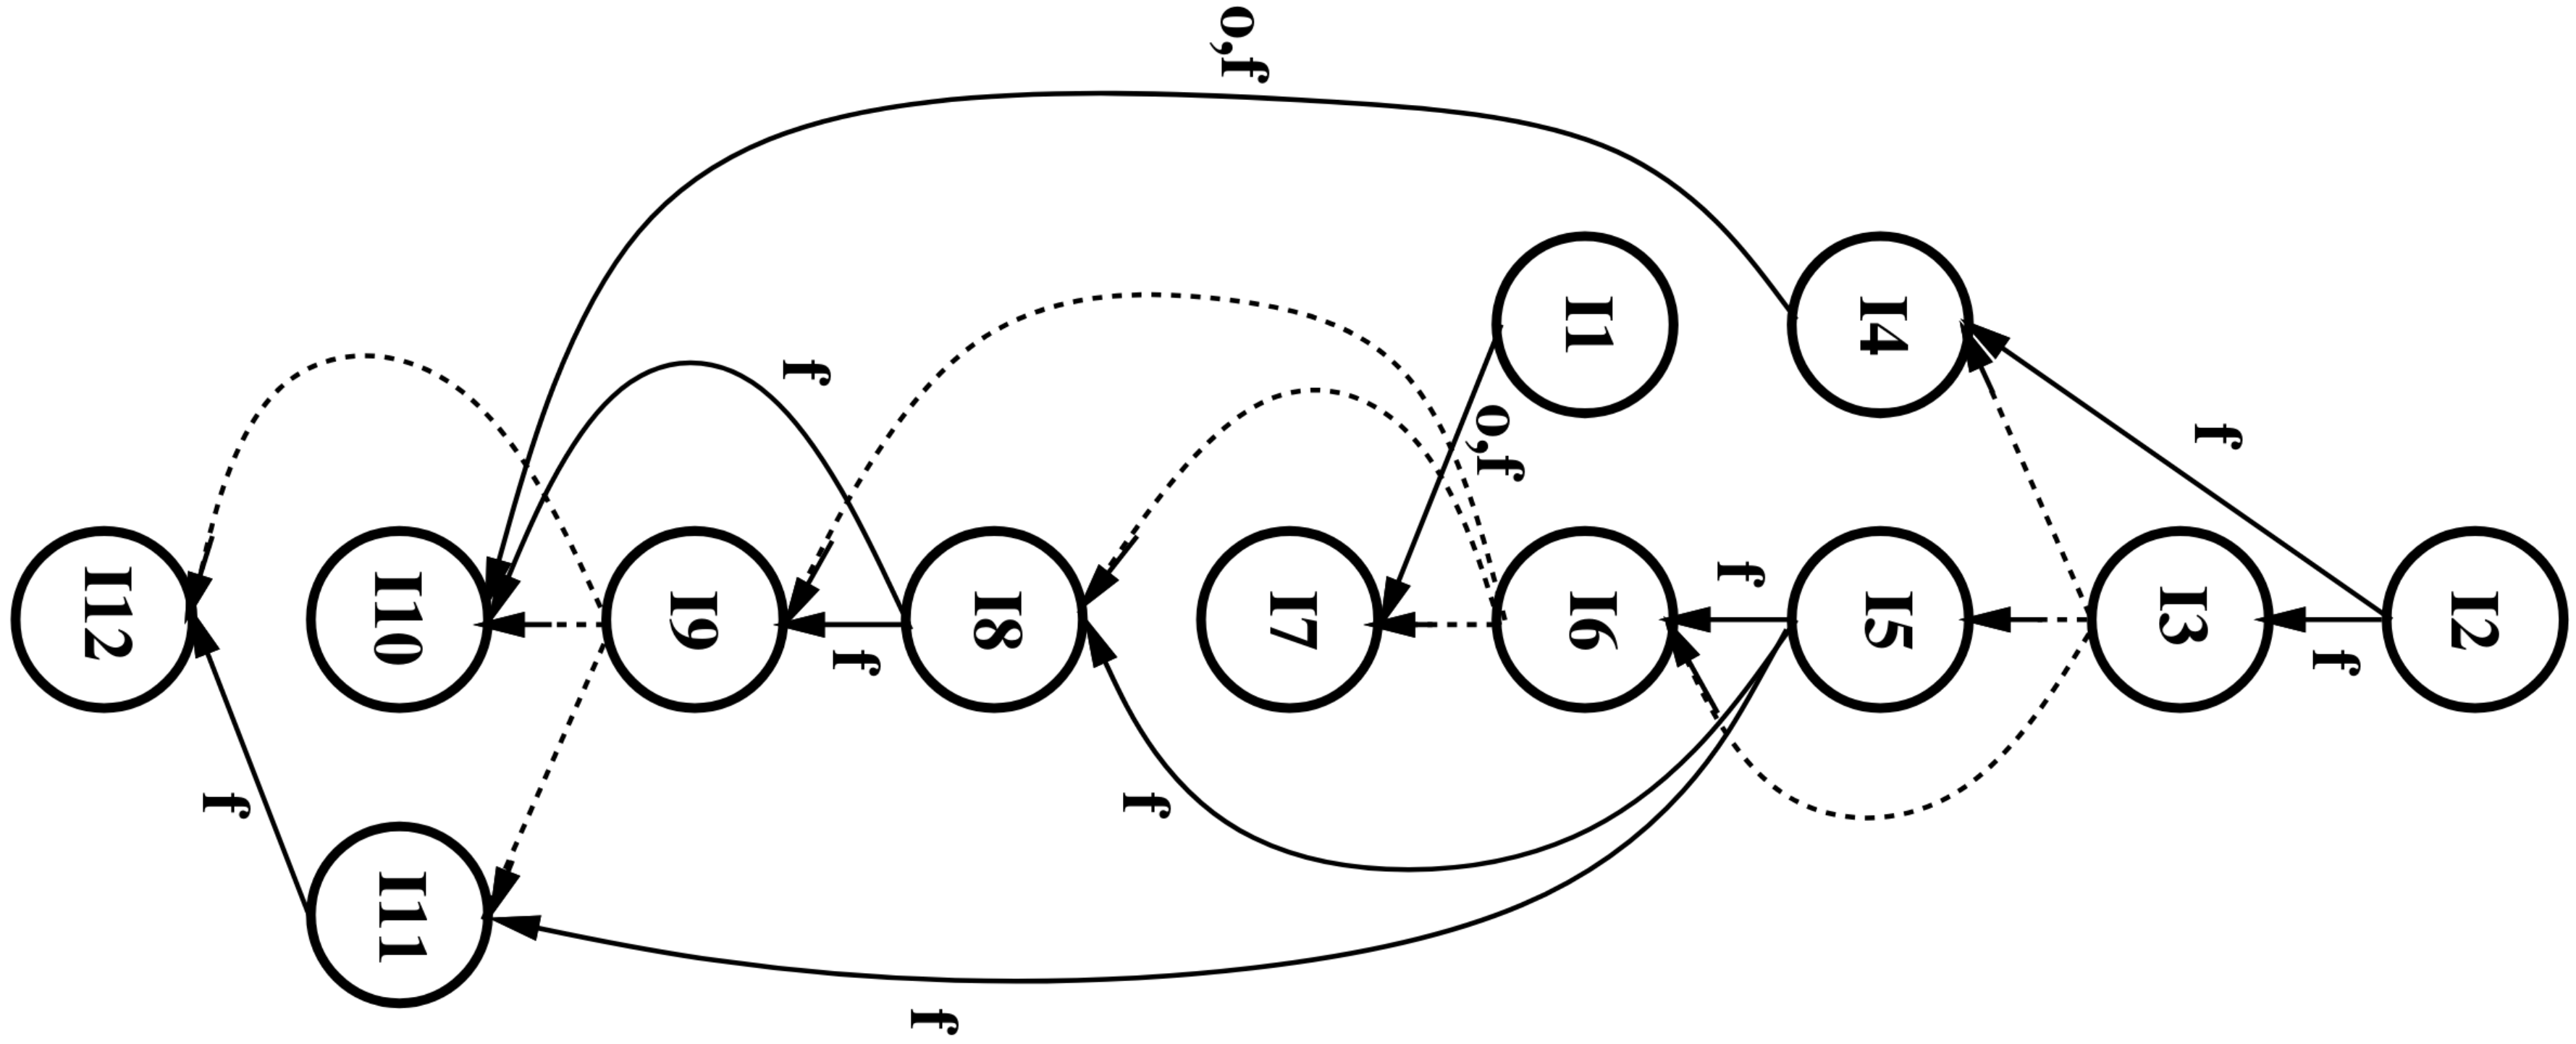
\includegraphics[width=\linewidth, angle=90]{src/figure/image/restricted_cfg.png}

            \caption[Dependence Graph for Restricted Code Percolation]{Dependence Graph for Restricted Code Percolation. Courtesy of Chang et al.~\cite{chang95}.}
            \label{fig:restric_cfg}
\end{figure}
    \end{minipage}\hfill
    \begin{minipage}{.46\textwidth}
    \begin{figure}[H]
            \centering
            \resizebox{1\textwidth}{!}{
            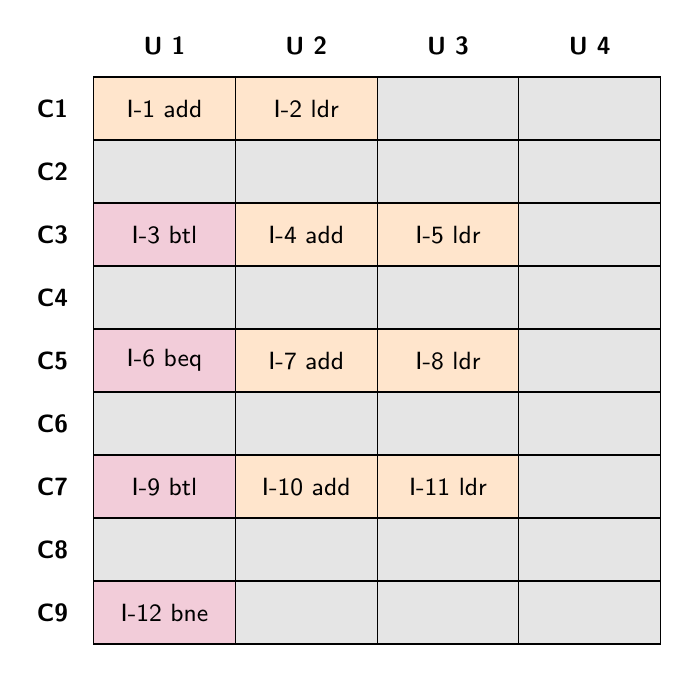
\begin{tikzpicture}[font=\sffamily, scale=1]
\def\cellwidth{1.8}
\def\cellheight{0.8}

\newlength{\cellwidthLength}
\setlength{\cellwidthLength}{\cellwidth cm}
\newlength{\cellheightLength}
\setlength{\cellheightLength}{\cellheight cm}

\tikzstyle{ALU} = [fill=orange!20, draw=black, rectangle, minimum width=\cellwidthLength, minimum height=\cellheightLength]
\tikzstyle{LOAD} = [fill=orange!20, draw=black, rectangle, minimum width=\cellwidthLength, minimum height=\cellheightLength]
\tikzstyle{BRANCH} = [fill=purple!20, draw=black, rectangle, minimum width=\cellwidthLength, minimum height=\cellheightLength]
\tikzstyle{EMPTY} = [fill=gray!20, draw=black, rectangle, minimum width=\cellwidthLength, minimum height=\cellheightLength]

\def\numcycles{9}
\def\numunits{4}

\foreach \i in {1,...,\numcycles} {
    \foreach \j in {1,...,\numunits} {
        \pgfmathsetmacro{\x}{(\j - 1) * \cellwidth}
        \pgfmathsetmacro{\y}{-\i * \cellheight}
        \draw[EMPTY] (\x cm, \y cm) rectangle ++(\cellwidthLength, \cellheightLength);
    }
}

\foreach \j in {1,...,\numunits} {
    \pgfmathsetmacro{\x}{(\j - 1) * \cellwidth + 0.5 * \cellwidth}
    \node at (\x cm, 0.5 * \cellheight cm) {\small\textbf{U \j}};
}

\foreach \i in {1,...,\numcycles} {
    \pgfmathsetmacro{\y}{-\i * \cellheight + 0.5 * \cellheight}
    \node[anchor=east] at (-0.2 cm, \y cm) {\small\textbf{C\i}};
}


% Cycle 1
\pgfmathsetmacro{\y}{-1 * \cellheight}
\draw[ALU] (0 cm, \y cm) rectangle ++(\cellwidthLength, \cellheightLength) node[pos=.5] {\small I-1 add};
\draw[LOAD] (\cellwidth cm, \y cm) rectangle ++(\cellwidthLength, \cellheightLength) node[pos=.5] {\small I-2 ldr};

% Cycle 3
\pgfmathsetmacro{\y}{-3 * \cellheight}
\draw[BRANCH] (0 cm, \y cm) rectangle ++(\cellwidthLength, \cellheightLength) node[pos=.5] {\small I-3 btl};
\draw[ALU] (\cellwidth cm, \y cm) rectangle ++(\cellwidthLength, \cellheightLength) node[pos=.5] {\small I-4 add};
\draw[LOAD] (2 * \cellwidth cm, \y cm) rectangle ++(\cellwidthLength, \cellheightLength) node[pos=.5] {\small I-5 ldr};

% Cycle 5
\pgfmathsetmacro{\y}{-5 * \cellheight}
\draw[BRANCH] (0 cm, \y cm) rectangle ++(\cellwidthLength, \cellheightLength) node[pos=.5] {\small I-6 beq};
\draw[ALU] (\cellwidth cm, \y cm) rectangle ++(\cellwidthLength, \cellheightLength) node[pos=.5] {\small I-7 add};
\draw[LOAD] (2 *\cellwidth cm, \y cm) rectangle ++(\cellwidthLength, \cellheightLength) node[pos=.5] {\small I-8 ldr};

% Cycle 7
\pgfmathsetmacro{\y}{-7 * \cellheight}
\draw[BRANCH] (0 cm, \y cm) rectangle ++(\cellwidthLength, \cellheightLength) node[pos=.5] {\small I-9 btl};
\draw[ALU] (\cellwidth cm, \y cm) rectangle ++(\cellwidthLength, \cellheightLength) node[pos=.5] {\small I-10 add};
\draw[LOAD] (2 * \cellwidth cm, \y cm) rectangle ++(\cellwidthLength, \cellheightLength) node[pos=.5] {\small I-11 ldr};

% Cycle 9
\pgfmathsetmacro{\y}{-9 * \cellheight}
\draw[BRANCH] (0 cm, \y cm) rectangle ++(\cellwidthLength, \cellheightLength) node[pos=.5] {\small I-12 bne};

\foreach \i in {1,...,\numcycles} {
    \foreach \j in {1,...,\numunits} {
        \pgfmathsetmacro{\x}{(\j - 1) * \cellwidth}
        \pgfmathsetmacro{\y}{-\i * \cellheight}
        \draw (\x cm, \y cm) rectangle ++(\cellwidthLength, \cellheightLength);
    }
}

\end{tikzpicture} 
        }
        \caption[Schedule for Restricted Code Percolation]{Under Restricted Code Percolation, we take nice cycles to execute an unrolled loop iteration. Due to the strict restrictions, the schedule tableau is sparse.}
        \label{fig:restricted_motion}
\end{figure}
    \end{minipage}
\end{center} 
Under Restricted Code Percolation, the compiler is not able to schedule long latency instructions such as the load instruction \texttt{I5} earlier since it may cause an exception. Additionally, we are limited when moving for example \texttt{I7}. Although its data dependencies are satisfied by the previously scheduled \texttt{I1}, its destination register \texttt{r2} is part of \texttt{live-out(I6)} on which \texttt{I7} is control dependent on. 

%%% Bringmann %%%
\subsubsection{Safe Speculation Model}
Safe Speculation~\cite{bringmannMH95} is an extension to Restricted Code Percolation which relaxes Restriction 2 in certain cases. Safe speculation preserves the \textit{avoid erros} property by employing compile-time program analysis to formally exclude the occurrence of exceptions during run time. Typically, this may include speculative loads in cases where the compiler can prove that the load will never raise an exception, for example by checking the boundaries of an allocated memory array. Other examples are division operations where there is formal proof that we may never attempt to divide by zero. Although it comes with an additional compile-time cost, it does not require additional hardware nor does it introduce the risk of false results which are inherent to for example \textit{ignore errors} speculations.  

\subsubsection{General Code Percolation}
General Code Percolation belongs to the category of \textit{ignore errors}~\cite{bringmannMH95} which lifts Restriction 2 by ignoring exceptions. To this end, it requires a non-excepting counterpart for any excepting instruction that we want to execute speculatively. This may include memory instructions, integer divide, and all floating-point arithmetic. These special instructions can be moved above control-dependent branches a long as they respect Restriction 1. However, as we ignore the occurring exception conditions, the program is valid to produce an incorrect under General Code Percolation. These errors can arise from different conditions. If a non-excepting load instruction tries to access an invalid address, the result loaded into the destination register will be garbage. If this value of the load is used, it will likely cause errors or actual exceptions. In the same manner, non-excepting integer division and floating-point instructions can cause unpredictable behavior.  The same applies to store operations, yet, compilers are typically more conservative with stores since it requires complex memory disambiguation analysis which oftentimes cannot be proven. The effects of General Code Percolation on the dependence graph can be seen in figure~\ref{fig:general_cfg}. 

\begin{center}
    \begin{minipage}{.52\textwidth}
        \begin{figure}[H]
            \centering
            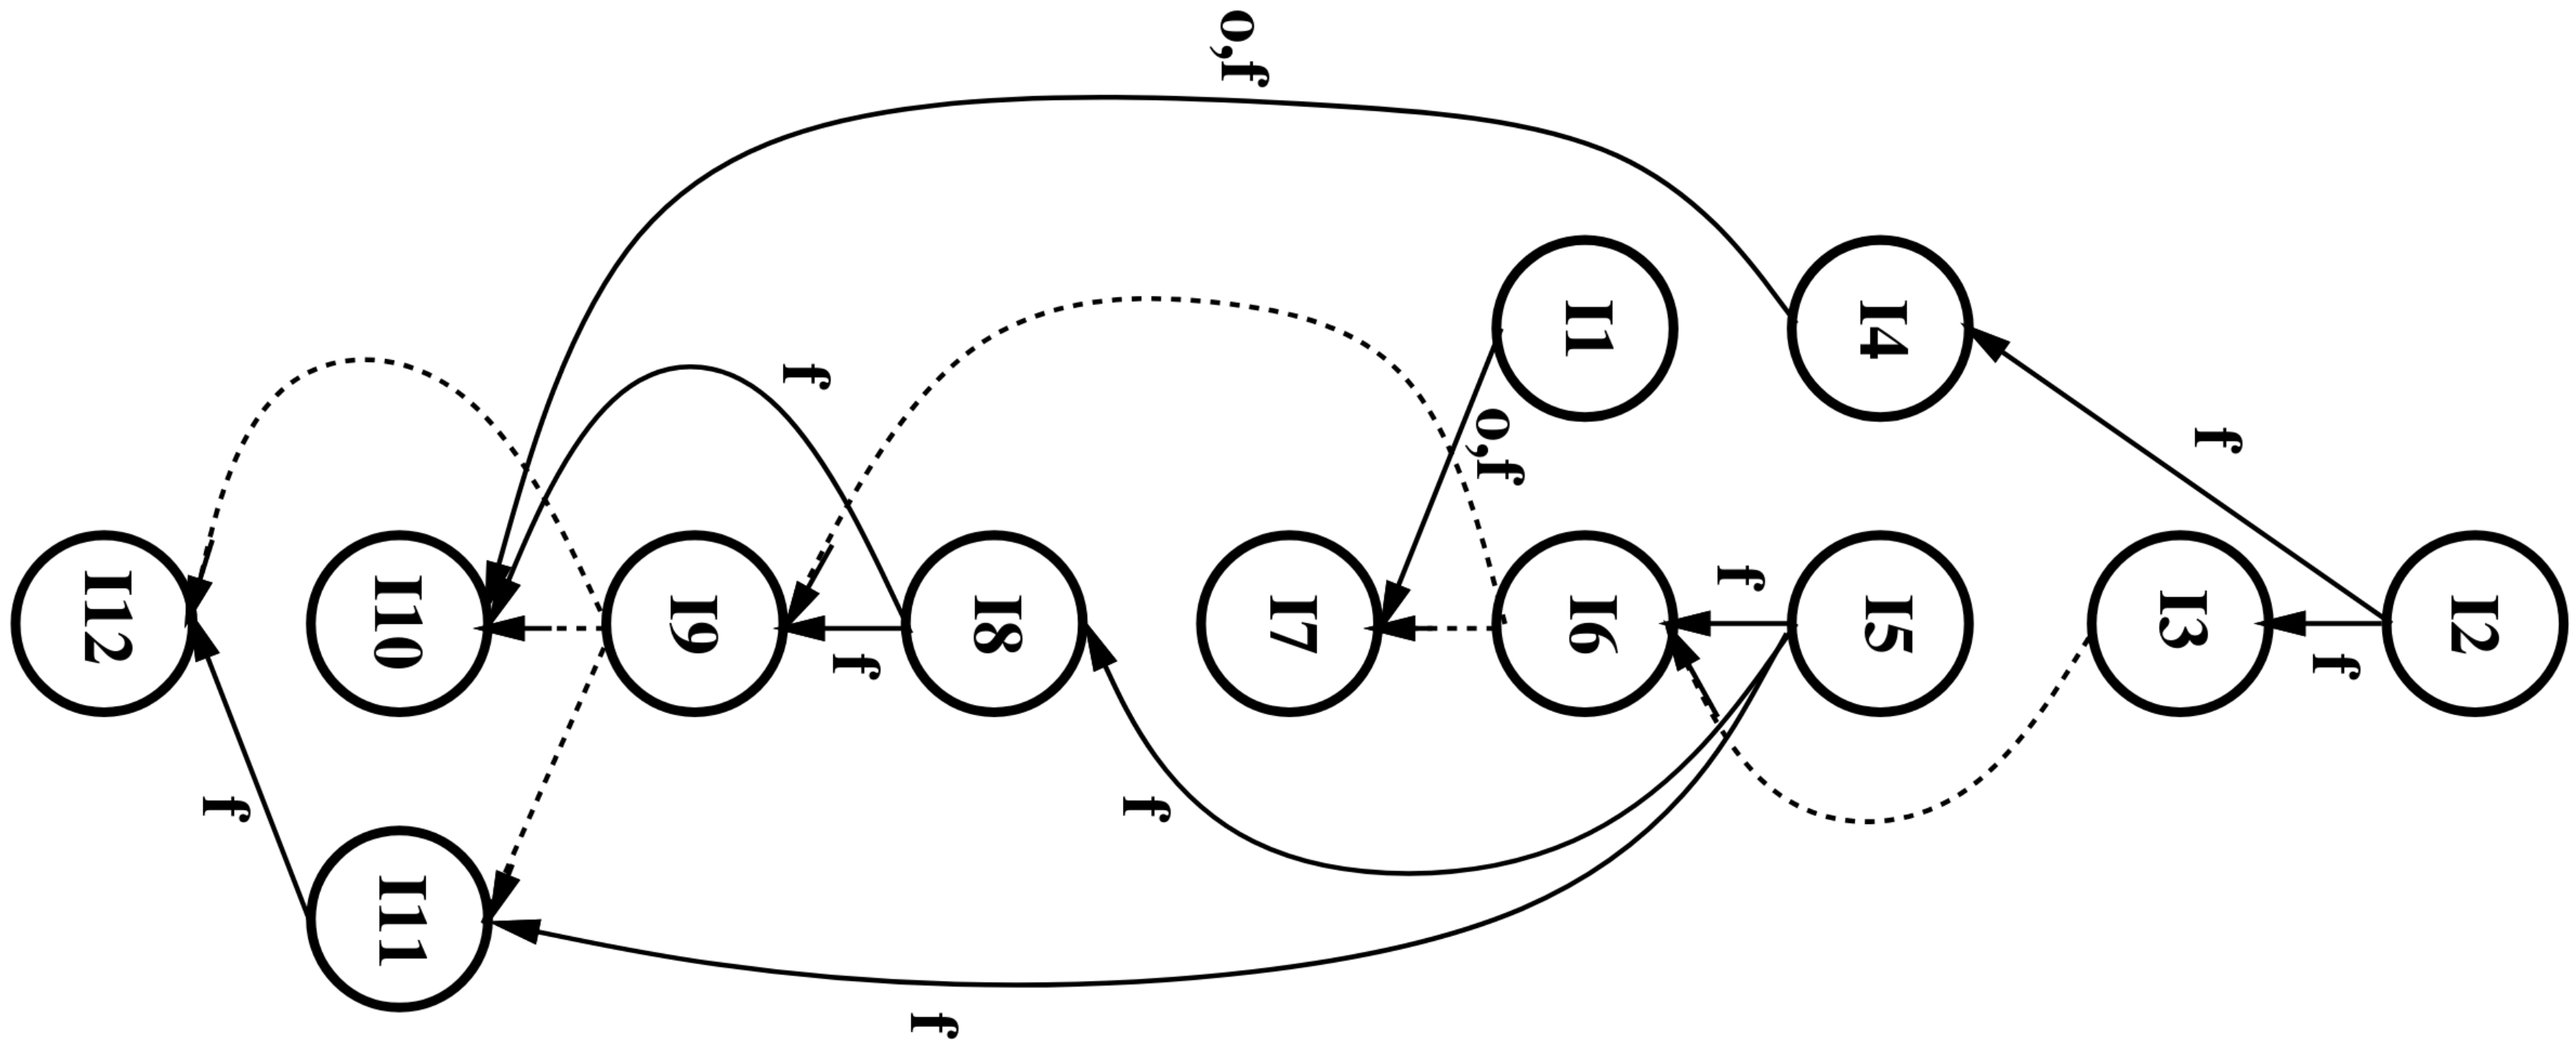
\includegraphics[width=\linewidth, angle=90]{src/figure/image/general_cfg.png}

            \caption[Dependence Graph for General Code Percolation]{Dependence Graph for General Code Percolation. Courtesy of Chang et al.~\cite{chang95}.}
            \label{fig:general_cfg}
\end{figure}
    \end{minipage}\hfill
    \begin{minipage}{.46\textwidth}
\begin{figure}[H]
            \centering
            \resizebox{1\textwidth}{!}{
            \begin{tikzpicture}[font=\sffamily, scale=1]
\def\cellwidth{1.8}
\def\cellheight{0.8}

% Define lengths with units
%\newlength{\cellwidthLength}
\setlength{\cellwidthLength}{\cellwidth cm}
%\newlength{\cellheightLength}
\setlength{\cellheightLength}{\cellheight cm}

\tikzstyle{ALU} = [fill=orange!20, draw=black, rectangle, minimum width=\cellwidthLength, minimum height=\cellheightLength]
\tikzstyle{LOAD} = [fill=orange!20, draw=black, rectangle, minimum width=\cellwidthLength, minimum height=\cellheightLength]
\tikzstyle{BRANCH} = [fill=purple!20, draw=black, rectangle, minimum width=\cellwidthLength, minimum height=\cellheightLength]
\tikzstyle{EMPTY} = [fill=gray!20, draw=black, rectangle, minimum width=\cellwidthLength, minimum height=\cellheightLength]

\def\numcycles{5}
\def\numunits{4}

\foreach \i in {1,...,\numcycles} {
    \foreach \j in {1,...,\numunits} {
        \pgfmathsetmacro{\x}{(\j - 1) * \cellwidth}
        \pgfmathsetmacro{\y}{-\i * \cellheight}
        \draw[EMPTY] (\x cm, \y cm) rectangle ++(\cellwidthLength, \cellheightLength);
    }
}

\foreach \j in {1,...,\numunits} {
    \pgfmathsetmacro{\x}{(\j - 1) * \cellwidth + 0.5 * \cellwidth}
    \node at (\x cm, 0.5 * \cellheight cm) {\small\textbf{U \j}};
}

\foreach \i in {1,...,\numcycles} {
    \pgfmathsetmacro{\y}{-\i * \cellheight + 0.5 * \cellheight}
    \node[anchor=east] at (-0.2 cm, \y cm) {\small\textbf{C\i}};
}

% Cycle 1
\pgfmathsetmacro{\y}{-1 * \cellheight}
\draw[ALU] (0 cm, \y cm) rectangle ++(\cellwidthLength, \cellheightLength) node[pos=.5] {\small I-1 add};
\draw[LOAD] (\cellwidth cm, \y cm) rectangle ++(\cellwidthLength, \cellheightLength) node[pos=.5] {\small I-2 ldr};
\draw[LOAD] (2 * \cellwidth cm, \y cm) rectangle ++(\cellwidthLength, \cellheightLength) node[pos=.5] {\small I-5 ldr};

% Cycle 3
\pgfmathsetmacro{\y}{-3 * \cellheight}
\draw[BRANCH] (0 cm, \y cm) rectangle ++(\cellwidthLength, \cellheightLength) node[pos=.5] {\small I-3 btl};
\draw[ALU] (\cellwidth cm, \y cm) rectangle ++(\cellwidthLength, \cellheightLength) node[pos=.5] {\small I-4 add};
\draw[LOAD] (2 * \cellwidth cm, \y cm) rectangle ++(\cellwidthLength, \cellheightLength) node[pos=.5] {\small I-8 ldr};
\draw[LOAD] (3 * \cellwidth cm, \y cm) rectangle ++(\cellwidthLength, \cellheightLength) node[pos=.5] {\small I-11 ldr};

% Cycle 4
\pgfmathsetmacro{\y}{-4 * \cellheight}
\draw[BRANCH] (0 cm, \y cm) rectangle ++(\cellwidthLength, \cellheightLength) node[pos=.5] {\small I-6 beq};

% Cycle 5
\pgfmathsetmacro{\y}{-5 * \cellheight}
\draw[ALU] (0 cm, \y cm) rectangle ++(\cellwidthLength, \cellheightLength) node[pos=.5] {\small I-7 add};
\draw[BRANCH] (\cellwidth cm, \y cm) rectangle ++(\cellwidthLength, \cellheightLength) node[pos=.5] {\small I-9 btl};
\draw[ALU] (2 *\cellwidth cm, \y cm) rectangle ++(\cellwidthLength, \cellheightLength) node[pos=.5] {\small I-10 add};
\draw[BRANCH] (3 *\cellwidth cm, \y cm) rectangle ++(\cellwidthLength, \cellheightLength) node[pos=.5] {\small I-12 bne};

\foreach \i in {1,...,\numcycles} {
    \foreach \j in {1,...,\numunits} {
        \pgfmathsetmacro{\x}{(\j - 1) * \cellwidth}
        \pgfmathsetmacro{\y}{-\i * \cellheight}
        \draw (\x cm, \y cm) rectangle ++(\cellwidthLength, \cellheightLength);
    }
}

\end{tikzpicture} 
        }
        \caption[Schedule for General Code Percolation]{A valid superblock schedule under General Code Percolation. By lifting restriction 2, we are able to schedule long-latency instructions such as \texttt{I5}, \texttt{I8}, and \texttt{I11} earlier at the cost of input-dependent output errors.}
        \label{fig:general_motion}
\end{figure}
    \end{minipage}
\end{center} 

Control dependencies can now be removed if the destination register of an instruction if not in \texttt{live-out()} of the above control flow instruction. For example, this applies to the load instruction \texttt{I8} which is control dependent on branch instruction \texttt{I6}, yet, the destination register \texttt{r6} of \texttt{I8} is not live in the taken-section of \texttt{I6}. Hence, the load can be scheduled before the branch, but it may cause an exception as the pointer in register \texttt{r5} may have been null. However, ignoring eventual exceptions allows us to reduce the number of control dependencies to six compared to the nine in the restricted example in section~\ref{rest_code_per}. A resulting schedule can be seen in figure~\ref{fig:general_motion}. An unrolled iteration is now scheduled to take five cycles instead of the previous nine. 

\subsubsection{Boosting Code Percolation}
When employing Boosting Code Percolation, the compiler can speculatively schedule instructions that violate both Restriction 1 and Restriction 2. The model belongs to the so-called \textit{resolve errors}~\cite{bringmannMH95} category, meaning the result of the program will ultimately be the same as a non-speculatively scheduled version. To this end, we require hardware support of the target system which allows to delay the commitment of a speculatively executed instruction until the branch it is dependent on commits. This includes a \textit{shadow register file}~\cite{10.1145/325096.325160} which will hold boosted instructions until the result of the respective branch is known. For speculative store instructions, a \textit{shadow store buffer} is required. The hardware will keep track of boosted instructions. This includes for example one or multiple bits which indicate how many branches the instructions were moved upwards. The previously described superblock structure is vital to the following parts, as we can assume that boosted instructions are part of the not-taken path of the branch. For example, in case the branch commits while boosted instructions are still in the pipeline, they are somewhat not executed speculatively anymore and we can remove their boosted label, hence converting them to normal instructions. In case the branch was taken, the boosted instructions in the pipeline will be squashed. However, boosted instructions will also finish before their branch commits. In this case, the result of the instruction will be held in a shadow register. In a superblock, we can simply copy the shadow value into the real register or the write buffer in case of stores if the branch was not taken. In the taken case, we destroy the shadow values and have to start executing the branch target code. We overcome Restriction 2 by delaying the handling of exceptions caused by boosted instructions until their branch commits. If the branch is taken, we can ignore all exceptions of boosted instructions, since they were never supposed to be executed anyway. In case the branch was not taken and we encounter one more exception, we have to roll back and squash the pipeline, and start re-executing the not-taken code sequentially until the first exception occurs.
\begin{center}
    \begin{minipage}{.52\textwidth}
        \begin{figure}[H]
            \centering
            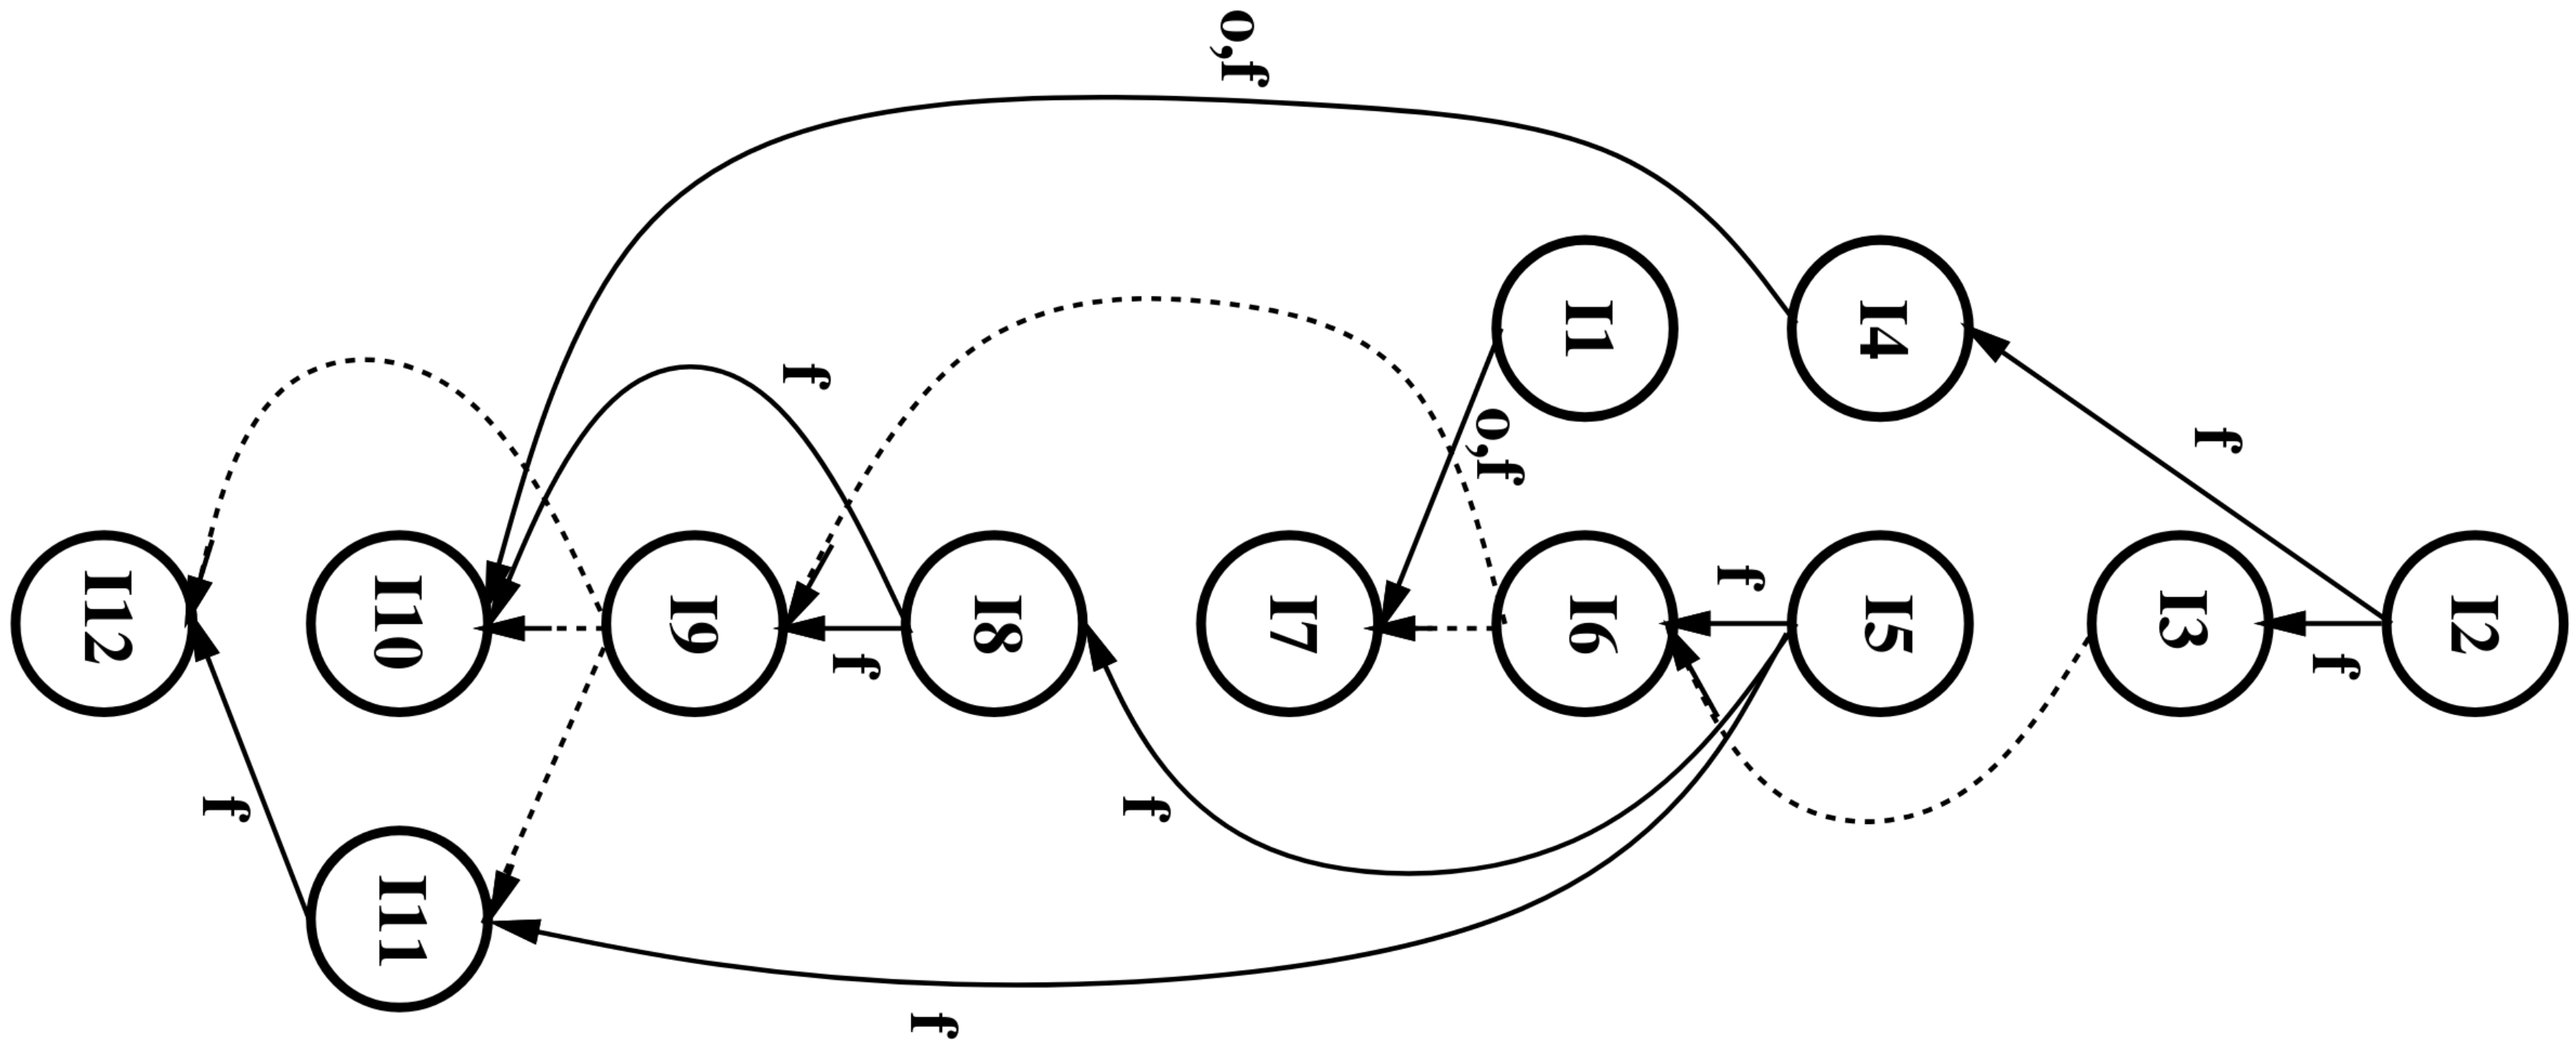
\includegraphics[width=\linewidth, angle=90]{src/figure/image/general_cfg.png}

            \caption[Dependence Graph for Boosting Code Percolation]{Dependence Graph for Boosting Code Percolation. Courtesy of Chang et al.~\cite{chang95}.}
            \label{fig:boosting_cfg}
\end{figure}
    \end{minipage}\hfill
    \begin{minipage}{.46\textwidth}
\begin{figure}[H]
            \centering
            \resizebox{1\textwidth}{!}{
            \begin{tikzpicture}[font=\sffamily, scale=1]
\def\cellwidth{1.8}
\def\cellheight{0.8}

%\newlength{\cellwidthLength}
\setlength{\cellwidthLength}{\cellwidth cm}
%\newlength{\cellheightLength}
\setlength{\cellheightLength}{\cellheight cm}

\tikzstyle{ALU} = [fill=orange!20, draw=black, rectangle, minimum width=\cellwidthLength, minimum height=\cellheightLength]
\tikzstyle{LOAD} = [fill=orange!20, draw=black, rectangle, minimum width=\cellwidthLength, minimum height=\cellheightLength]
\tikzstyle{BRANCH} = [fill=purple!20, draw=black, rectangle, minimum width=\cellwidthLength, minimum height=\cellheightLength]
\tikzstyle{EMPTY} = [fill=gray!20, draw=black, rectangle, minimum width=\cellwidthLength, minimum height=\cellheightLength]

\def\numcycles{5}
\def\numunits{4}

\foreach \i in {1,...,\numcycles} {
    \foreach \j in {1,...,\numunits} {
        \pgfmathsetmacro{\x}{(\j - 1) * \cellwidth}
        \pgfmathsetmacro{\y}{-\i * \cellheight}
        \draw[EMPTY] (\x cm, \y cm) rectangle ++(\cellwidthLength, \cellheightLength);
    }
}

\foreach \j in {1,...,\numunits} {
    \pgfmathsetmacro{\x}{(\j - 1) * \cellwidth + 0.5 * \cellwidth}
    \node at (\x cm, 0.5 * \cellheight cm) {\small\textbf{U \j}};
}

\foreach \i in {1,...,\numcycles} {
    \pgfmathsetmacro{\y}{-\i * \cellheight + 0.5 * \cellheight}
    \node[anchor=east] at (-0.2 cm, \y cm) {\small\textbf{C\i}};
}

% Cycle 1
\pgfmathsetmacro{\y}{-1 * \cellheight}
\draw[ALU] (0 cm, \y cm) rectangle ++(\cellwidthLength, \cellheightLength) node[pos=.5] {\small I-1 add};
\draw[LOAD] (\cellwidth cm, \y cm) rectangle ++(\cellwidthLength, \cellheightLength) node[pos=.5] {\small I-2 ldr};
\draw[LOAD] (2 * \cellwidth cm, \y cm) rectangle ++(\cellwidthLength, \cellheightLength) node[pos=.5] {\small I-5 ldr};

% Cycle 2
\pgfmathsetmacro{\y}{-2 * \cellheight}
\draw[ALU] (0 cm, \y cm) rectangle ++(\cellwidthLength, \cellheightLength) node[pos=.5] {\small I-7 add};

% Cycle 3
\pgfmathsetmacro{\y}{-3 * \cellheight}
\draw[BRANCH] (0 cm, \y cm) rectangle ++(\cellwidthLength, \cellheightLength) node[pos=.5] {\small I-3 btl};
\draw[ALU] (\cellwidth cm, \y cm) rectangle ++(\cellwidthLength, \cellheightLength) node[pos=.5] {\small I-4 add};
\draw[LOAD] (2 * \cellwidth cm, \y cm) rectangle ++(\cellwidthLength, \cellheightLength) node[pos=.5] {\small I-8 ldr};
\draw[LOAD] (3 * \cellwidth cm, \y cm) rectangle ++(\cellwidthLength, \cellheightLength) node[pos=.5] {\small I-11 ldr};

% Cycle 4
\pgfmathsetmacro{\y}{-4 * \cellheight}
\draw[BRANCH] (0 cm, \y cm) rectangle ++(\cellwidthLength, \cellheightLength) node[pos=.5] {\small I-6 beq};

% Cycle 5
\pgfmathsetmacro{\y}{-5 * \cellheight}
\draw[BRANCH] (0 cm, \y cm) rectangle ++(\cellwidthLength, \cellheightLength) node[pos=.5] {\small I-9 btl};
\draw[ALU] (\cellwidth cm, \y cm) rectangle ++(\cellwidthLength, \cellheightLength) node[pos=.5] {\small I-10 add};
\draw[BRANCH] (2 *\cellwidth cm, \y cm) rectangle ++(\cellwidthLength, \cellheightLength) node[pos=.5] {\small I-12 bne};


\foreach \i in {1,...,\numcycles} {
    \foreach \j in {1,...,\numunits} {
        \pgfmathsetmacro{\x}{(\j - 1) * \cellwidth}
        \pgfmathsetmacro{\y}{-\i * \cellheight}
        \draw (\x cm, \y cm) rectangle ++(\cellwidthLength, \cellheightLength);
    }
}

\end{tikzpicture} 
        }
        \caption[Schedule for Boosting Code Percolation]{Schedule for Boosting Code Percolation}
        \label{fig:boosted_motion}
\end{figure}
    \end{minipage}
\end{center} 
The dependence graph resulting from Boosting Code Percolation can be seen in figure~\ref{fig:boosting_cfg}. When assuming hardware support for boosting instructions above one branch, the number of control dependencies in the superblock can be reduced to three. The scheduling freedom provided by the hardware support can be seen in figure~\ref{fig:boosted_motion}. For example, we can now schedule the increment instruction \texttt{I7} for the previously idle cycle two without the need for additional recovery code since the hardware will hold the value back until the branch of \texttt{I6} is committed and not taken. 

\subsubsection{Sentinel Scheduling}
Sentinel Scheduling~\cite{10.1145/161541.159765} is another model belonging to the \textit{resolve errors}~\cite{bringmannMH95} category. Sentinel scheduling exploits certain architectural features to detect and resolve exceptions caused by speculatively scheduled instructions. To his end, excepting instructions are split into two parts; the instruction itself which performs the operation, and a sentinel which will handle potentially occurring exceptions. The operation part can be moved above a branch as long as the sentinel remains in the \textit{home block} of the non-speculative control flow graph. Typically, we are able to remove sentinels recursively by exploiting the sentinel of an output-dependent instruction in the same home block, because this sentinel will report the exception of both instructions which makes it a so-called \textit{shared sentinel}. To enable sentinel scheduling, the hardware needs to provide additional support for the compiler to mark speculative instructions using a bit in the opcode. Additionally, the registers need to be extended with an exception tag to indicate any exception that occurred during execution. If a speculative instruction causes an exception, it is not immediately reported. In this case, the exception bit of the destination register is set and the program counter obtained from a history queue is copied into the data part of the register. In the following, if a given instruction uses one or more registers as a source that have their exception tag set, the first exception that has occurred in program order will be handled. For the case where a speculatively and potentially excepting instruction has no consumer in its home block, we need a dedicated sentinel instruction that takes a given register as a source operand and checks the exception tag. Essentially, this can be an arbitrary move instruction that takes the result of the speculative instruction as a source. 

\subsection{Profiling and Speculation}
In order to enable the compiler to enhance the schedule by speculating, we need to provide information about what input the programmer expects during run time and hence the most likely control flow behavior of the program. In this section, we will use the LLVM profiling infrastructure~\cite{llvm_profdata} to explore how profiling data can affect the program performance both in positive and negative ways, e.g. if the sampling data diverges from the actual input during run time. In our study, we want to compare a conservatively and aggressively speculative scheduled program~\cite{estes2014schedmachinemodel}. The compilation and profiling steps can be seen in the appendix section in listing~\ref{ls:makefile_specprof}. In LLVM, it is hard to restrict the compiler to one optimization, however, we try to minimize external influence by disabling common optimizations manually. We cannot use \texttt{-O0}, because it will also disable the \texttt{-enable-misched=true} which we have to use to enable machine-dependent scheduling decisions which likely will include speculations. We can instrument the program seen in listing~\ref{ls:ls_c_chang_full_default} to profile it using the \texttt{-fprofile-instr-generate}. Afterward, we can produce the profiling data by running the program. The code of listing~\ref{ls:build_node} is used to generate input data. Most importantly, we can specify the percentage of weight values that are positive, hence how frequently the branch deciding to subtract or add will be taken. For the analysis, we profile the application under the assumption that 99\% of the weights are positive.
\newpage 

\begin{center}
        \begin{lstlisting}[style=CStyle]
struct Node* build_list(int64_t N, double percent_positive) {
    struct Node* head = NULL;
    struct Node* current = NULL;
    int64_t i;

    for (i = 0; i < N; i++) {
        struct Node* new_node = (struct Node*)malloc(sizeof(struct Node));
        if (new_node == NULL) {
            fprintf(stderr, "Memory allocation failed %" PRId64 "\n", i);
            exit(EXIT_FAILURE);
        }

        if ((rand() / (double)RAND_MAX) < percent_positive) {
            new_node->wt = rand() % 100 + 1;
        } else {
            new_node->wt = -(rand() % 100 + 1);
        }
        new_node->next = NULL;

        if (head == NULL) {
            head = new_node;
            current = new_node;
        } else {
            current->next = new_node;
            current = new_node;
        }
    }
    return head;
}
\end{lstlisting}
        \captionsetup{type=listing}
        \captionof{lstlisting}[C Code for Input Data Generation]{C Code for Input Data Generation. We can specify the percentage of weight which are positive.}
        \label{ls:build_node}
\end{center}

In the following, we will compare the program compiled in three different ways while disabling most optimization as seen in listing~\ref{ls:makefile_specprof}. Initially, the program is compiled with no additional profiling data. Next, we compile the program again and pass the compiler profiling data which assumes 99\% positive weights using the \texttt{-fprofile-instr-use} option. For one program, we enable \texttt{-enable-misched} which enables target-specific scheduling decisions. Lastly, we compile one version without these additional scheduling optimizations. In the following experiment, we execute each version five times and take the average execution time measured as can be seen in listing~\ref{ls:run_nodes}.
\begin{center}
        \begin{lstlisting}[style=CStyle]
clock_gettime(CLOCK_MONOTONIC, &start_time);
    while (ptr != NULL) {
        count++;
        if(ptr->wt < 0) {
            weight -= ptr->wt;
        } else {
            weight += ptr->wt;
        }
        struct Node* temp = ptr;
        ptr = ptr->next;
        free(temp);
    }
clock_gettime(CLOCK_MONOTONIC, &end_time);
\end{lstlisting}
        \captionsetup{type=listing}
        \captionof{lstlisting}[C Code for Running the Benchmarking]{Instrumented C Code for processing the nodes.}
        \label{ls:run_nodes}
\end{center}
The following plot in figure~\ref{fig:plot_specdiv} shows the execution time for processing $6\times10^8$ nodes of the three versions. While we always profile and hence compile under the assumption that 99\% of the weights are positive, we increase the percentage of negative weights on the x-axis.  
\begin{center}
    \begin{minipage}{.87\textwidth}
        \begin{figure}[H]
            \centering
            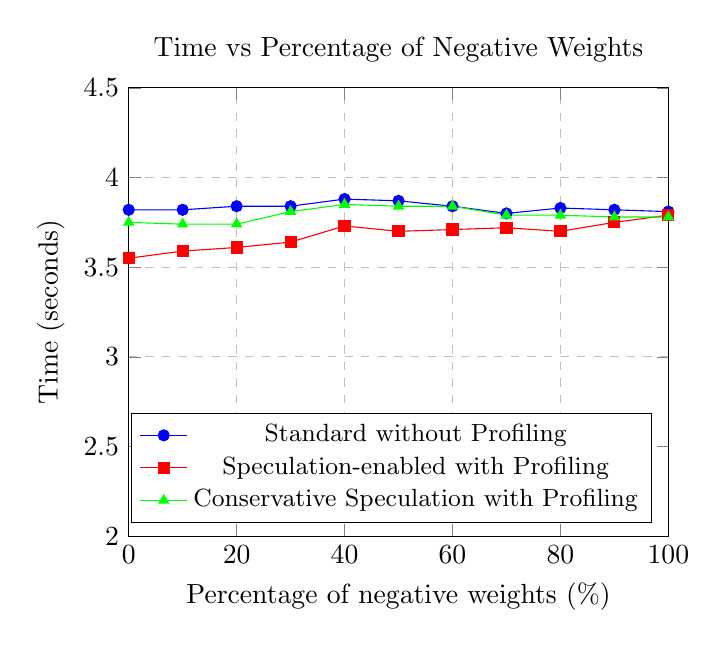
\begin{tikzpicture}
\begin{axis}[
    title={Time vs Percentage of Negative Weights},
    xlabel={Percentage of negative weights (\%)},
    ylabel={Time (seconds)},
    xmin=0, xmax=100,
    ymin=2, ymax=4.5,
    xtick={0,20,40,60,80,100},
    ytick={2,2.5,3,3.5,4,4.5},
    legend pos=south east,
    legend style={font=\small},
    ymajorgrids=true,
    xmajorgrids=true,
    grid style=dashed,
]

\addplot[color=blue, mark=*] coordinates {
    (0, 3.82)
    (10, 3.82)
    (20, 3.84)
    (30, 3.84)
    (40, 3.88)
    (50, 3.87)
    (60, 3.84)
    (70, 3.80)
    (80, 3.83)
    (90, 3.82)
    (100, 3.81)
};
\addlegendentry{Standard without Profiling}

\addplot[color=red, mark=square*] coordinates {
    (0, 3.55)
    (10, 3.59)
    (20, 3.61)
    (30, 3.64)
    (40, 3.73)
    (50, 3.70)
    (60, 3.71)
    (70, 3.72)
    (80, 3.70)
    (90, 3.75)
    (100, 3.79)
};
\addlegendentry{Speculation-enabled with Profiling}

\addplot[color=green, mark=triangle*] coordinates {
    (0, 3.75)
    (10, 3.74)
    (20, 3.74)
    (30, 3.81)
    (40, 3.85)
    (50, 3.84)
    (60, 3.84)
    (70, 3.79)
    (80, 3.79)
    (90, 3.78)
    (100, 3.78)
};
\addlegendentry{Conservative Speculation with Profiling}

\end{axis}
\end{tikzpicture}

            \caption[Execution Time with increased Input Data Divergence]{Execution Time with increased input data divergence during run time. The differences are marginal, yet, we can observe how the execution time of the speculative program is rising constantly while the standard program can recover after surpassing the 50\% negative weight mark.}
            \label{fig:plot_specdiv}
\end{figure}
    \end{minipage}
\end{center} 
We can observe how the differences are marginal. One possible explanation is the execution environment which is a superscalar x86 processor that features branch prediction which will certainly affect the outcome. In fact, in the conservative and standard plots, we can observe a small bump in execution time around the 50\% mark which may indicate that this is a configuration that is hard to predict. On the other hand, we can see how the speculation-enabled can not recover the original execution time. The experiment would be more meaningful on a VLIW processor where we are dealing with less noise coming from the hardware. 

\subsection{Attributes \texttt{likely} and \texttt{unlikely}}
LLVM and the respective \texttt{clang} compiler support numerous attributes that programmers can use to give hints to the compiler. In this case, \texttt{likely} and \texttt{unlikely}~\cite{clangsupportedsyntaxes} can be used to indicate if a branch will likely be taken or not. Similar to providing profiling data, this may enable the compiler to make better decisions during scheduling using the domain knowledge of the programmer. In our case, we may annotate the case where we have to process a negative weight as unlikely, as can be seen in listing~\ref{ls:lik_nodes}. However, in its current state, we could not observe any significant difference in execution time in our benchmarking setup. 
\begin{center}
        \begin{lstlisting}[style=CStyle]
while (ptr != NULL) {
    count++;
    @if (ptr->wt < 0) [[unlikely]] {@
        weight -= ptr->wt;
    } else {
        weight += ptr->wt;
    }
    ptr = ptr->next;
}

\end{lstlisting}
        \captionsetup{type=listing}
        \captionof{lstlisting}[C Code with \texttt{unlikely} Hint]{We can annotate the negative-case branch with \texttt{[[ unlikely ]]} to support the compiler during scheduling.}
        \label{ls:lik_nodes}
\end{center}
\newpage

